\chapter{Proposed Solution Concept}
\label{chap:solution-concept}

To successfully fulfil the defined objectives, we propose the solution described in this chapter. We will develop a robust framework capable of generating semantic segmentation masks for individual TILs from weak bounding box annotations. The high-level overview of architecture can be seen in figure \ref{fig:sc-main}. It can be split into three main parts (modules) each responsible for different tasks:

\begin{enumerate}
    \item \textbf{Image preprocessing module} will contain various image preprocessing techniques, such as normalization of images, artifacts removal, resizing and cropping.
    \item \textbf{Pseudo-label generating module} will be responsible for generating pseudo-labels in the form of segmentation masks.
    \item \textbf{Deep learning model} will use the preprocessed images and the generated pseudo-masks to make predictions.
\end{enumerate}

\begin{figure}[H]
    \begin{centering}
    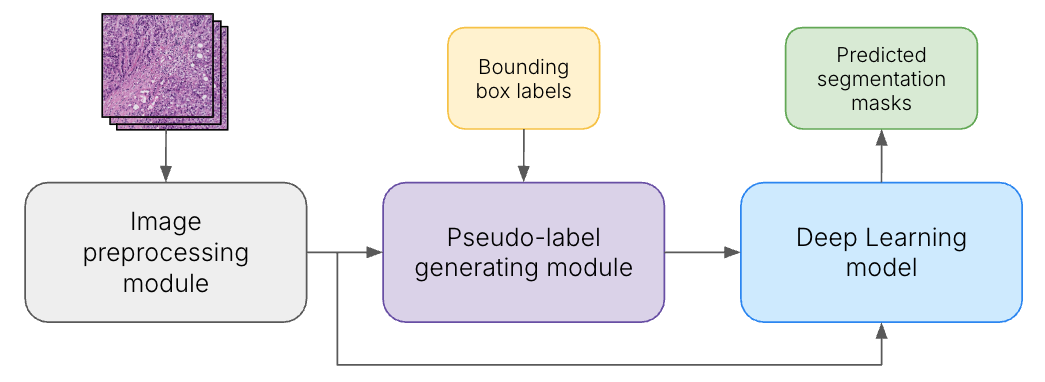
\includegraphics[width=14cm]{assets/images/sc-main.png}
    \par\end{centering}
    \caption{The high-level overview of the proposed architecture}
    \label{fig:sc-main}
\end{figure}

We describe each module in more detail in the following sections.

\section{Image Preprocessing Module}
\section{Pseudo-label Generating Module}
\section{Deep Learning Model}

